\documentclass[12pt,a4paper]{article}
\usepackage[utf8]{inputenc}
\usepackage{amsmath}
\usepackage{amsfonts}
\usepackage{amssymb}

\usepackage{placeins}
\usepackage{cmap} % для кодировки шрифтов в pdf
\usepackage[T1]{fontenc}
\usepackage{hhline}
\usepackage[unicode]{hyperref}
\usepackage{multirow}
\usepackage{array}
\usepackage{amsmath}
\usepackage{bm}
\usepackage{textcomp}
\usepackage[russian]{babel}
\usepackage{graphicx} % для вставки картинок
\usepackage{amssymb,amsfonts,amsmath,amsthm} % математические дополнения от АМС
\usepackage{indentfirst} % отделять первую строку раздела абзацным отступом тоже
% Поля
\usepackage{geometry}
\geometry{left=2cm}
\geometry{right=1.5cm}
\geometry{top=2.4cm}
\geometry{bottom=2.cm}

%%%%%%%%%%%%%%%%%%%%%%%%%%%%%%%     

\linespread{1.5} % полуторный интервал
\frenchspacing




\begin{document}
	
	\begin{titlepage}
		
		\begin{center}
			\begin{large}
				Санкт-Петербургский Политехнический университет\\ Петра Великого\\
				Физико-механический институт\\
			\end{large}
			\vspace{0.2cm}
			Высшая школа прикладной математики и вычислительной физики\\
			
		\end{center}
		
		\vspace{3cm}
		\begin{center}
			\textbf{Отчёт\\ по курсовой работе\\ по дисциплине\\ "Анализ данных с интервальной \\неопределенностью"}
		\end{center}
		
		\vspace{3cm}
		
		\vbox{%
			\hfill%
			\vbox{%
				\hbox{Выполнил студент:}%
				\hbox{\break}
				\hbox{Иванов Андрей Игоревич,}%
				\hbox{группа 5040102$\backslash$20201}%
				\hbox{\break}
				\hbox{\break}
				\hbox{Проверил:}
				\hbox{\break}
				\hbox{к.ф.-м.н., доцент}
				\hbox{Баженов Александр Николаевич}
			}%
		} 
		\vfill
		
		\begin{center}
			Санкт-Петербург, 2024
		\end{center}
	
	\end{titlepage}
	\tableofcontents
	\newpage
	
	\listoffigures
	\newpage
	
	\section{Постановка задачи}
            Дано множество частот мод показаний устройства, вычисляющего некоторое значение в зависимости от времени съема и длины волны входящего сигнала. Для дальнейшего анализа показаний полезно определить интервалы выбросов по всей временной выборке, так как известны эталонные значения частот мод для конкретных условий эксперимента, что может помочь в дальнейшей классификации природы результатов. Задача курсовой работы состоит в определении мультиинтервала частот мод (мультимоды) для показаний в различные моменты времени.
	\newpage
	
	\section{Теория}
            \subsection{Поиск мультимоды}
                Алгоритм поиска мультимоды выборки состоит из следующих шагов:
                \begin{enumerate}
                    \item Производится поиск моды для текущей выборки
                    \item Производится расширение интервала моды:
                    \begin{enumerate}
                        \item Интервал расширяется на фиксированную величину до тех пор, пока наибольшее из концевых значений частоты не превышает текущего максимального:
                        \begin{equation}
                            max(\mu) > max\{\mu(\underline{IH^k}), \mu(\overline{IH^k})\}
                        \end{equation}
                        $IH^k$ - расширяемый интервал на к-ом шаге.\\ 
                        \item Если условие остановки расширения не выполняется - границы интервала расширяются на фиксированную величину шага, предыдущие значения частоты зануляются.
                        \item В противном случае расширение интервала моды прекращается.
                    \end{enumerate}
                    \item В данной работе в качестве условия остановки поиска мультимоды выступало следующее условие:
                    \begin{equation}
                        max(\mu) > 2 * \overline{X}
                    \end{equation}
                    Данное условие было подобрано эмпирически. Если оно выполняется - на выходе генерируется множество расширенных интервалов частот мод, в противном случае - алгоритм возобновляет работу с первого шага.
                \end{enumerate}
                
	\newpage
	
	\section{Реализация}
		Лабораторная работа выполнена на языке Python 3.10, визуализация реализована при помощи загружаемого пакета MatPlotLib. Исходный код лабораторной работы находится на \href{https://github.com/Drusiand/SPbSTU_Interval_Analysis.git}{GitHub репозитории}.
	\newpage
	
	\section{Результаты}
            В качестве входных данных использовался файл "41000.txt".
                \begin{figure}[h!]
                    \centering
                    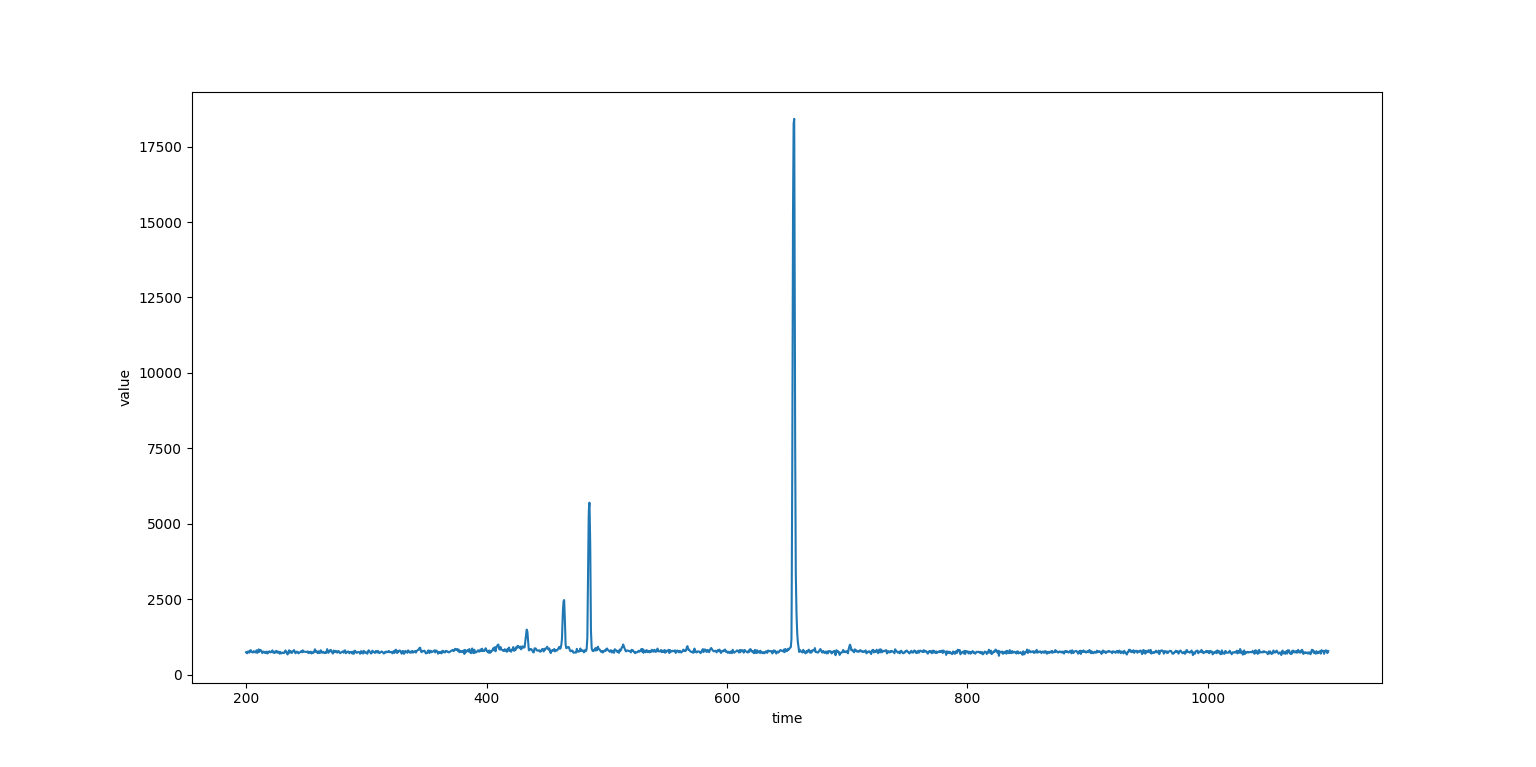
\includegraphics[width=0.95\linewidth]{sample_1_raw.png}
                    \caption{График первой выборки (столбец 17)}
                \end{figure}
                \FloatBarrier
                
                \begin{figure}[h!]
                    \centering
                    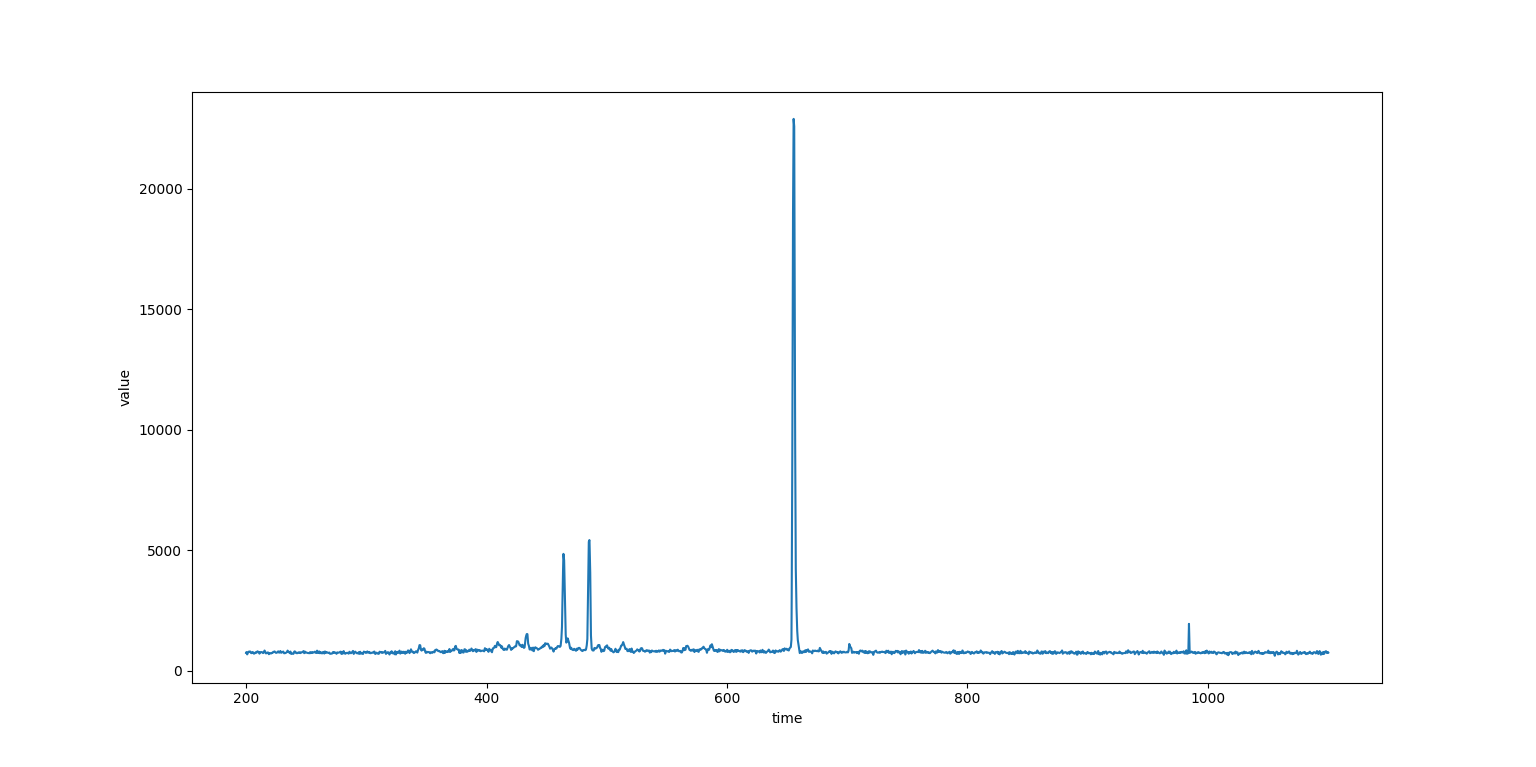
\includegraphics[width=0.95\linewidth]{sample_2_raw.png}
                    \caption{График второй выборки (столбец 59)}
                \end{figure}
                \FloatBarrier
                
                \begin{figure}[h!]
                    \centering
                    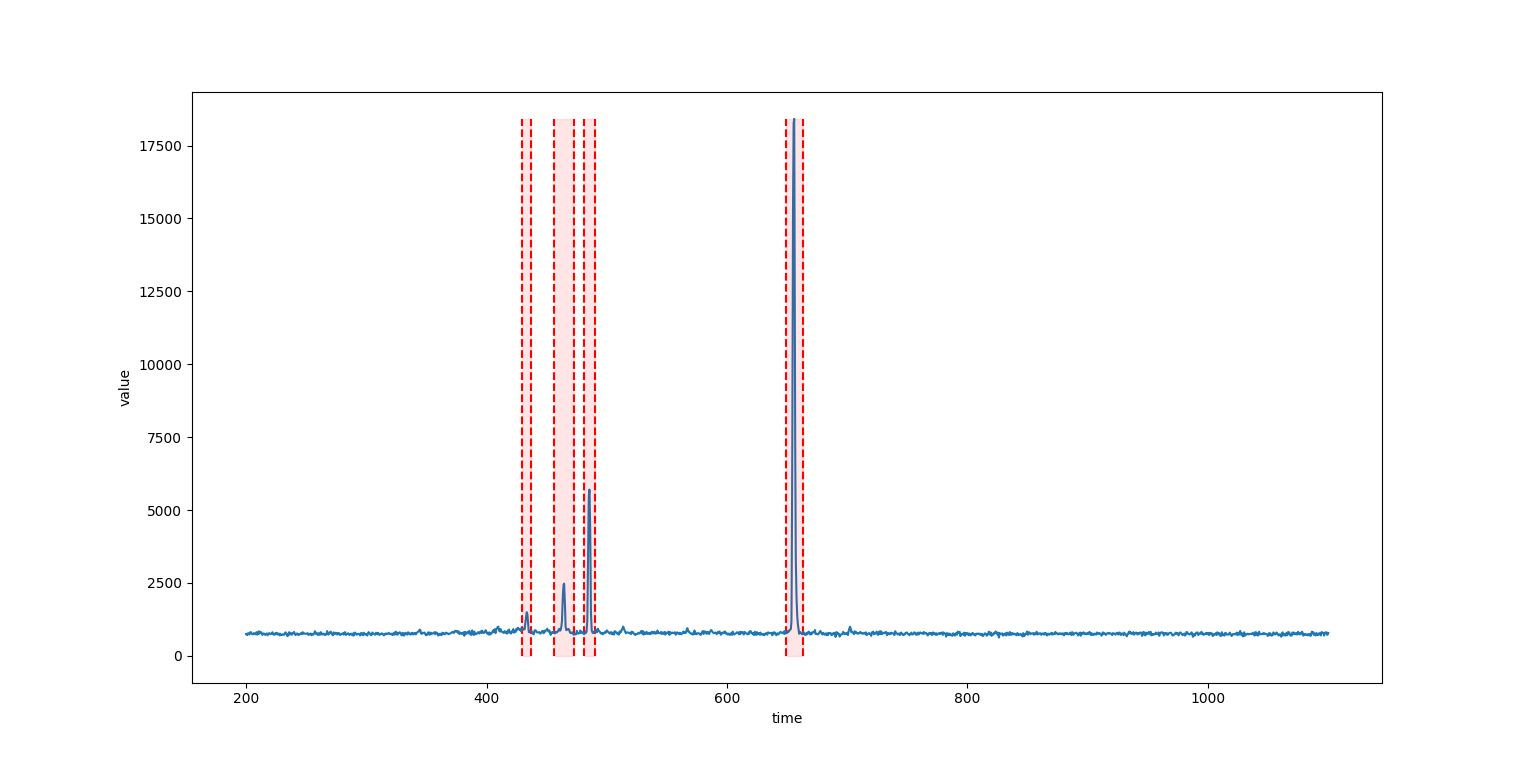
\includegraphics[width=0.95\linewidth]{sample_1.png}
                    \caption{График первой выборки с выделенной мультимодой}
                \end{figure}
                \FloatBarrier
                
                \begin{figure}[h!]
                    \centering
                    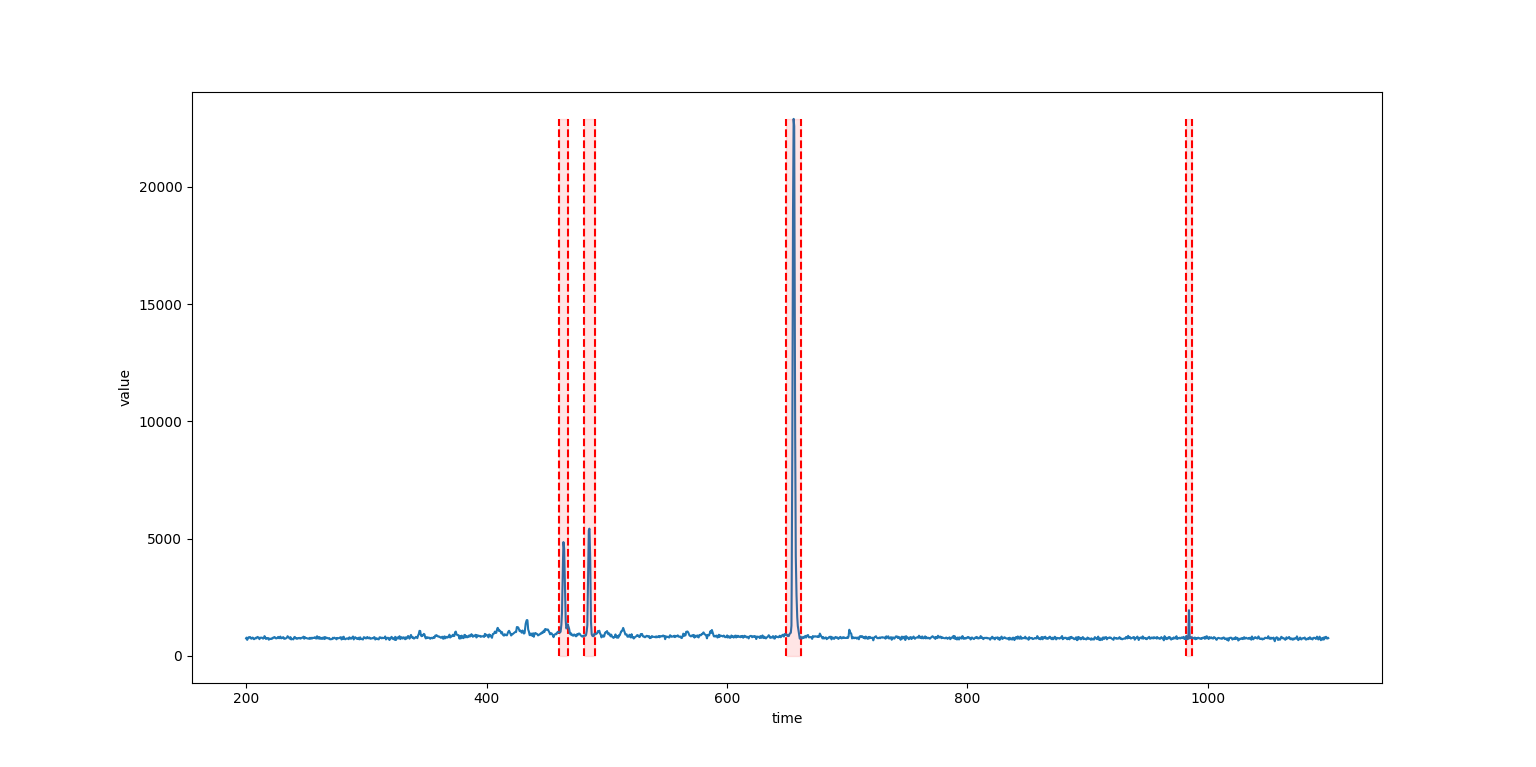
\includegraphics[width=0.95\linewidth]{sample_2.png}
                    \caption{График второй выборки с выделенной мультимодой}
                \end{figure}
                \FloatBarrier

            
                \begin{figure}[h!]
                    \centering
                    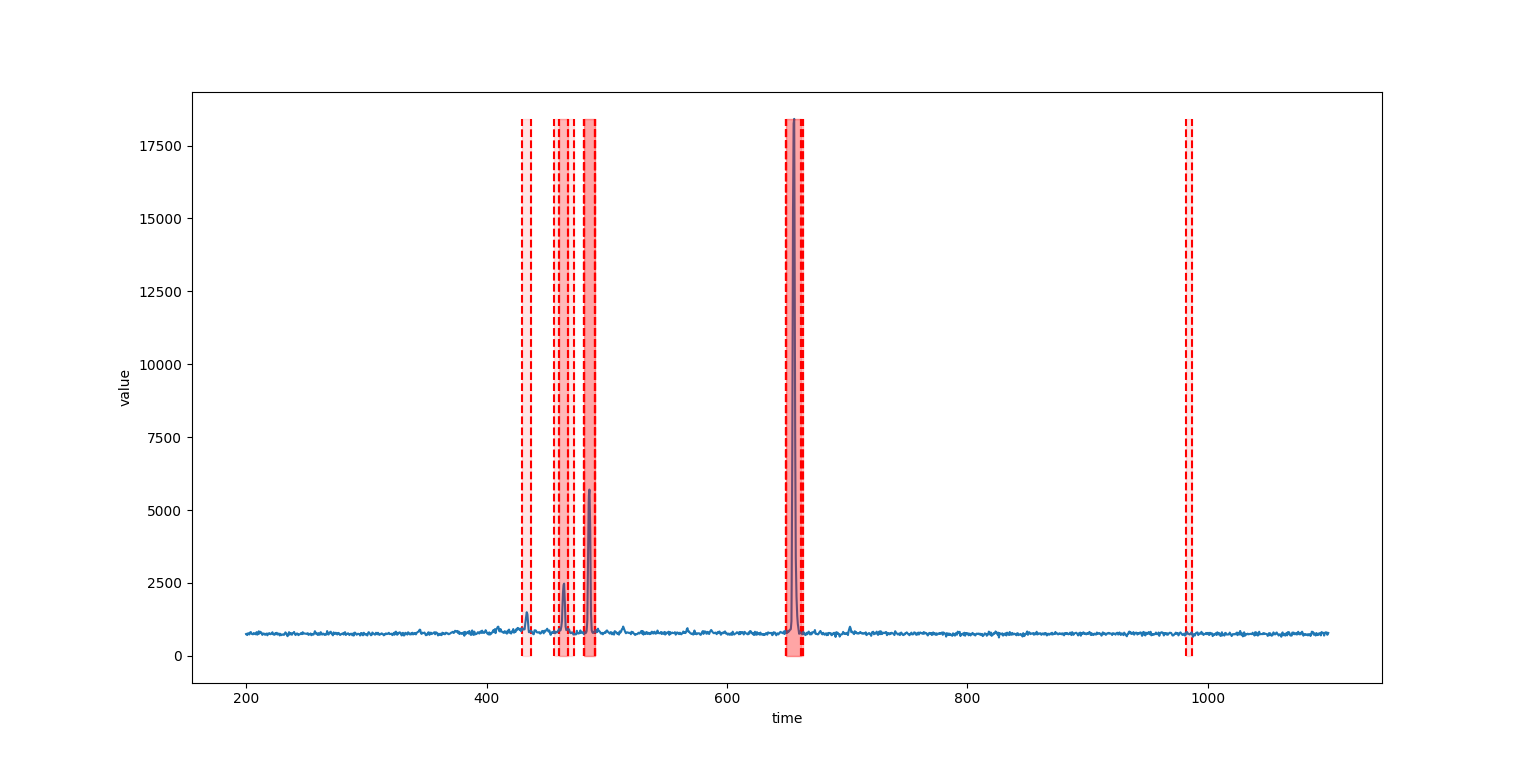
\includegraphics[width=0.95\linewidth]{sample_1_intersection.png}
                    \caption{График первой выборки с выделенной объединенной мультимодой}
                \end{figure}
                \FloatBarrier
    
                \begin{figure}[h!]
                    \centering
                    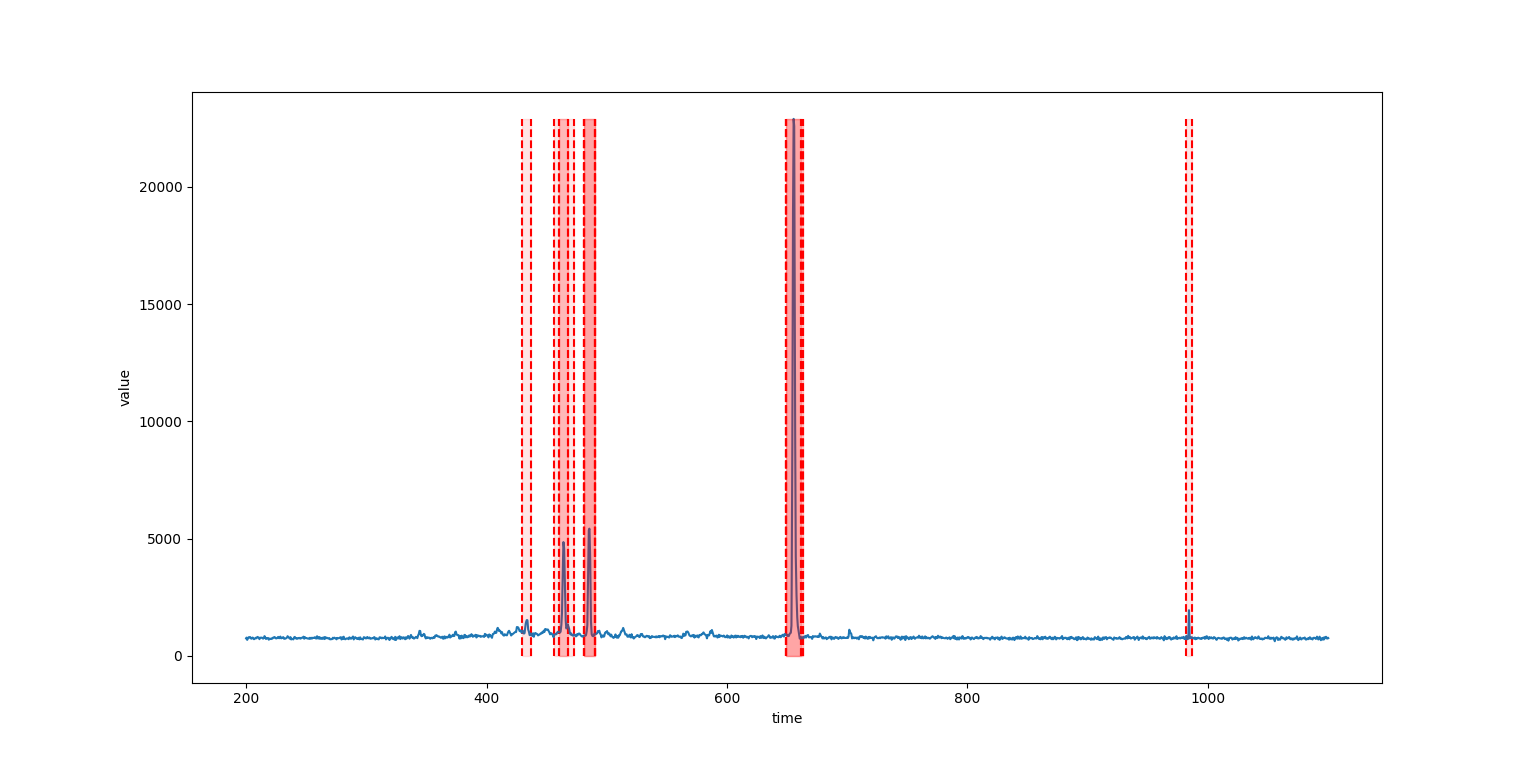
\includegraphics[width=0.95\linewidth]{sample_2_intersection.png}
                    \caption{График второй выборки с выделенной объединенной мультимодой}
                \end{figure}
                \FloatBarrier
        \clearpage
	\newpage

        \section{Обсуждение}
        Дальнейшее развитие работы состоит в поиске мультимоды глобальной выборки по всему набору данных с целью сопоставления с эталонными (табличными значениями). Для достижения наибольшей точности вычисления необходимо доработать алгоритм поиска с более точным обнаружением границ. Для удобства работы с подобными задачами следует реализовать библиотеку работы с мультиинтервалами, как можно больше семантически абстрагированную от прикладной области.
        
\end{document}